{\let\clearpage\relax \chapter{Grafiken}}
\begin{figure}[htb]
	\centering
	\begin{minipage}[t]{0.45\textwidth}
		\centering
		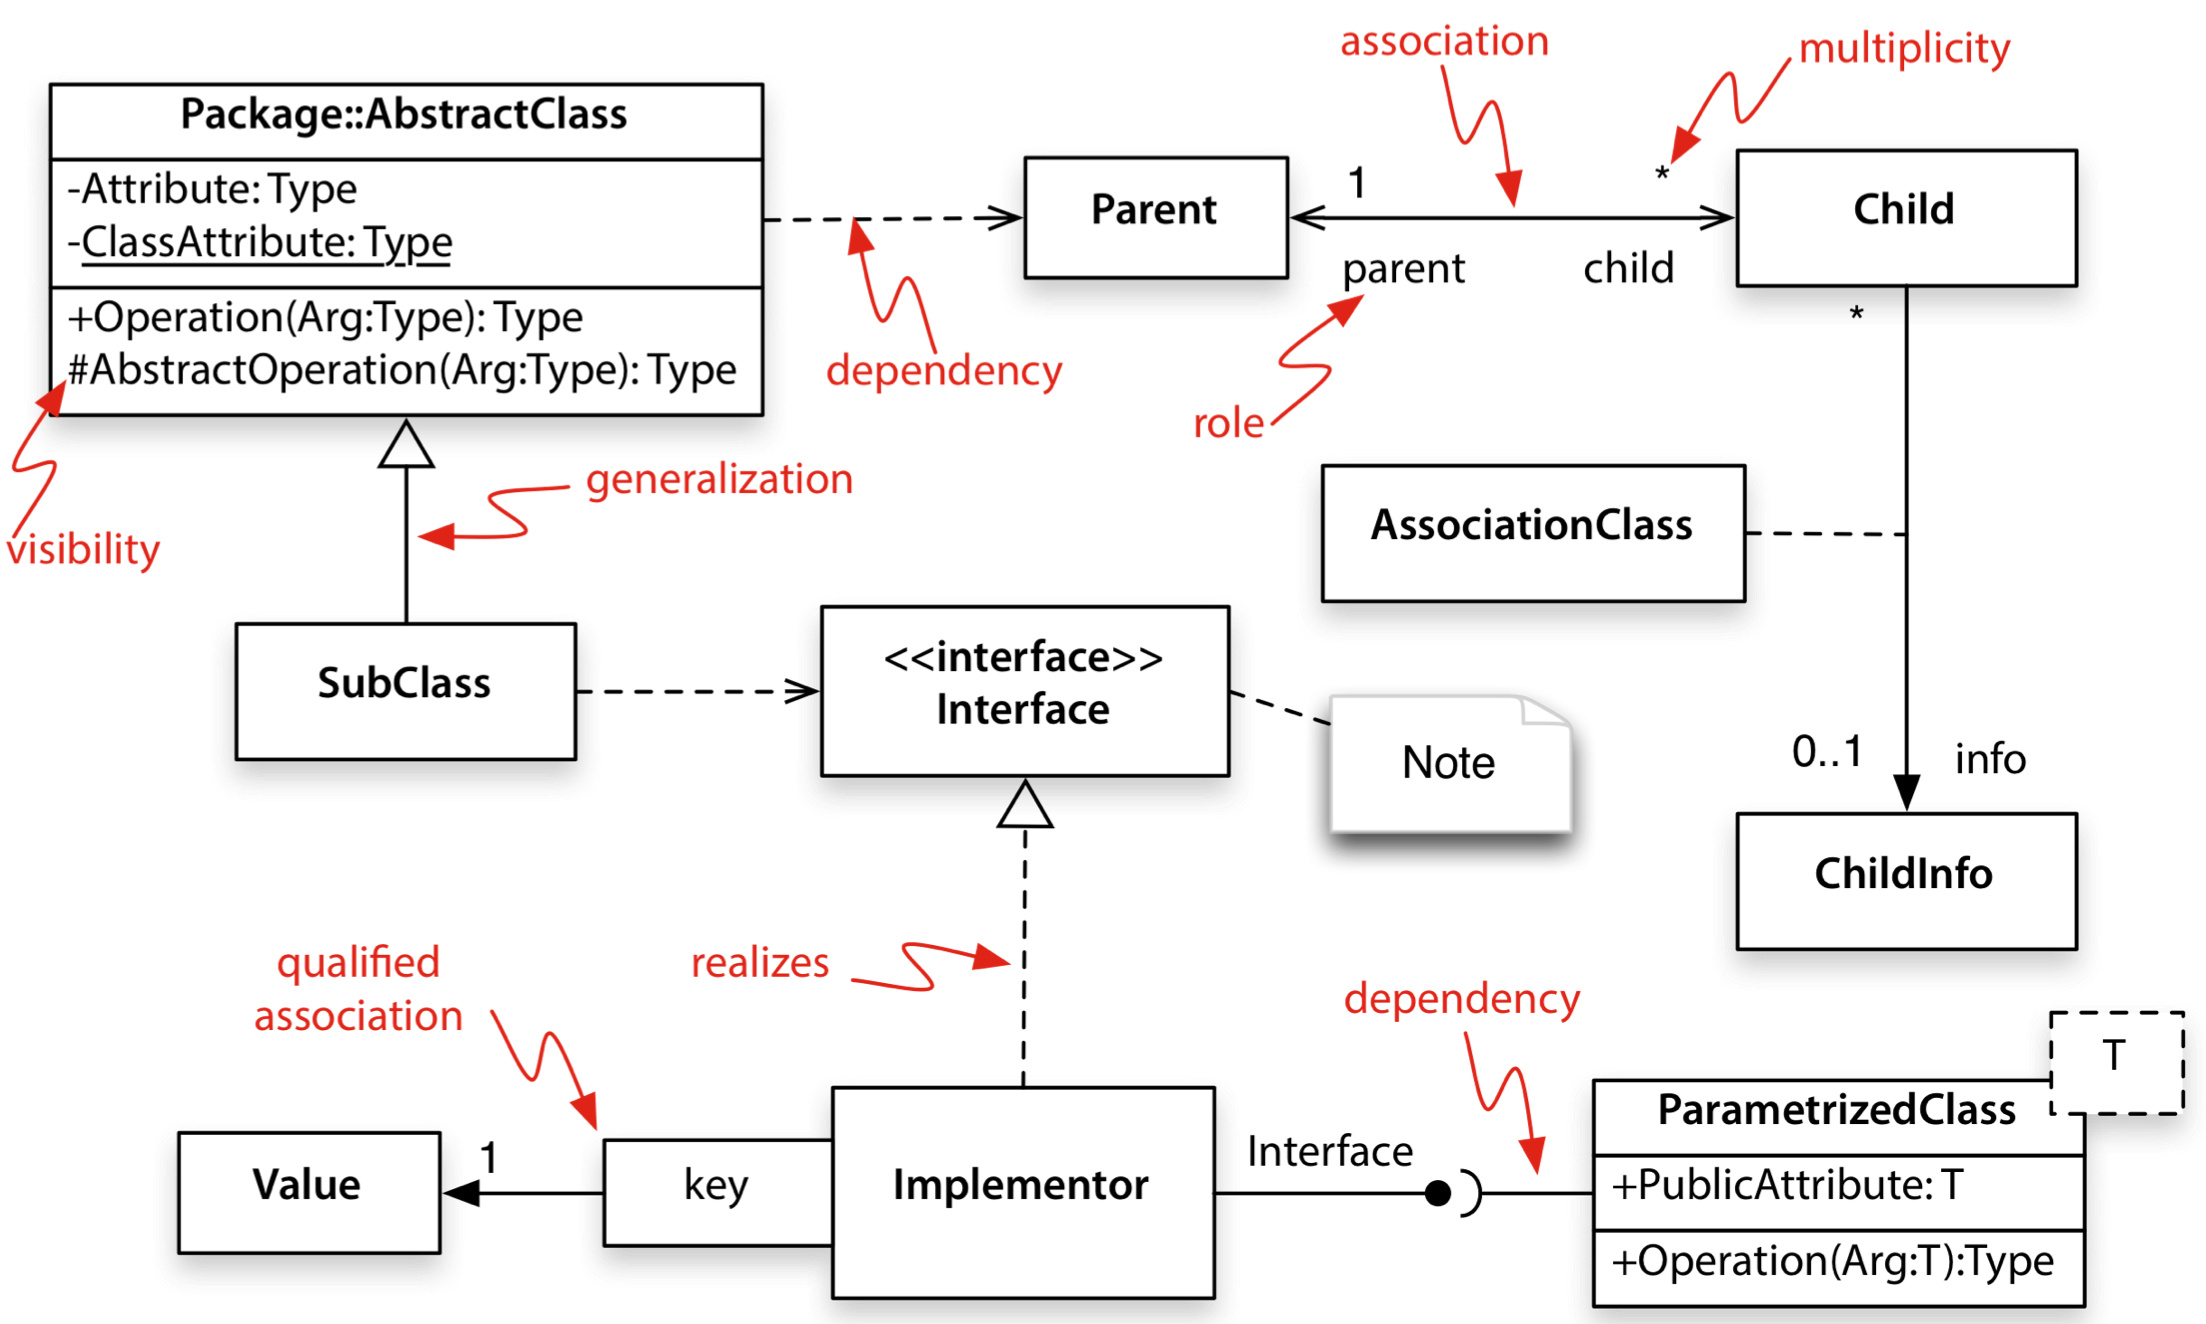
\includegraphics[width=0.9\textwidth]{images/uml}
		\label{fig:uml_notation}
		\caption{UML Notation}
	\end{minipage}% <- sonst wird hier ein Leerzeichen eingefügt
	\hfill
	\begin{minipage}[t]{0.45\textwidth}
		\centering
		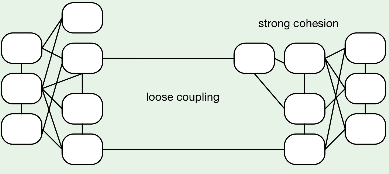
\includegraphics[width=0.9\textwidth]{images/loose_coupling}
		\label{fig:loose_coupling}
		\caption{loose coupling / strong cohesion}
	\end{minipage}
\end{figure}

\begin{figure}[htb]
	\centering
	\begin{minipage}[t]{0.45\linewidth}
		\centering
		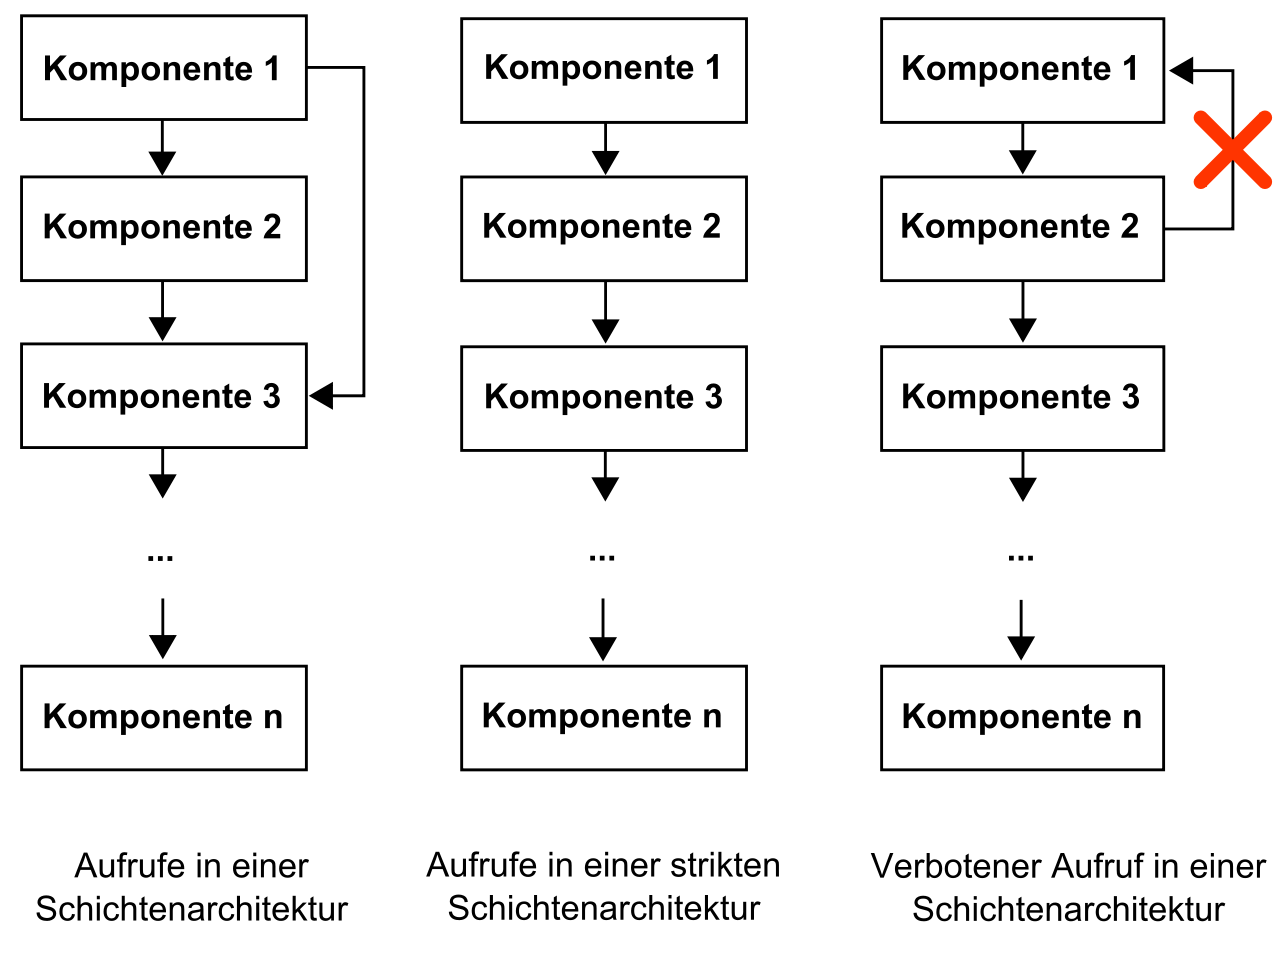
\includegraphics[width=0.9\textwidth]{images/layers}
		\label{fig:layers}
		\caption{Layers}
	\end{minipage}% <- sonst wird hier ein Leerzeichen eingefügt
	\hfill
	\begin{minipage}[t]{0.45\linewidth}
		\centering
		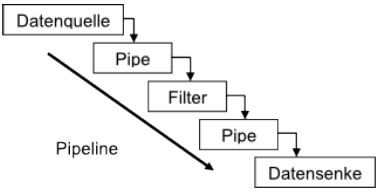
\includegraphics[width=0.9\textwidth]{images/pipes_filters}
		\label{fig:pipes_filters}
		\caption{Pipes and Filters}
	\end{minipage}
\end{figure}

\begin{figure}[htb]
	\centering
	\begin{minipage}[t]{0.45\linewidth}
		\centering
		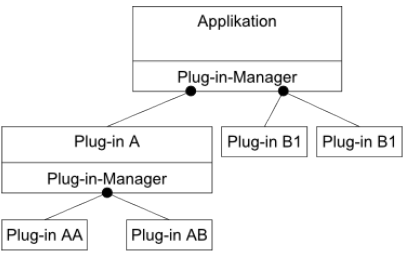
\includegraphics[width=0.9\textwidth]{images/plugin}
		\label{fig:plugin}
		\caption{Plugin}
	\end{minipage}% <- sonst wird hier ein Leerzeichen eingefügt
	\hfill
	\begin{minipage}[t]{0.45\linewidth}
		\centering
		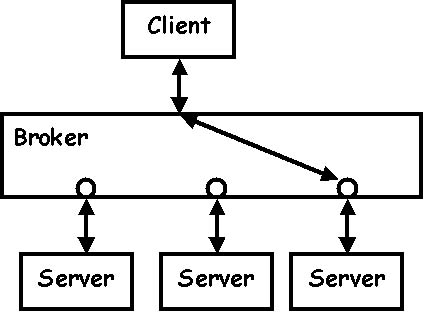
\includegraphics[width=0.9\textwidth]{images/broker}
		\label{fig:broker}
		\caption{Broker}
	\end{minipage}
\end{figure}

\begin{figure}[htb]
	\centering
	\begin{minipage}[t]{0.45\linewidth}
		\centering
		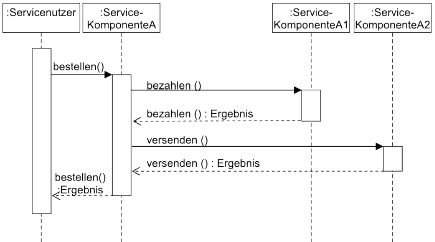
\includegraphics[width=0.9\textwidth]{images/soa}
		\label{fig:soa}
		\caption{SOA}
	\end{minipage}% <- sonst wird hier ein Leerzeichen eingefügt
	\hfill
	\begin{minipage}[t]{0.45\linewidth}
		\centering
		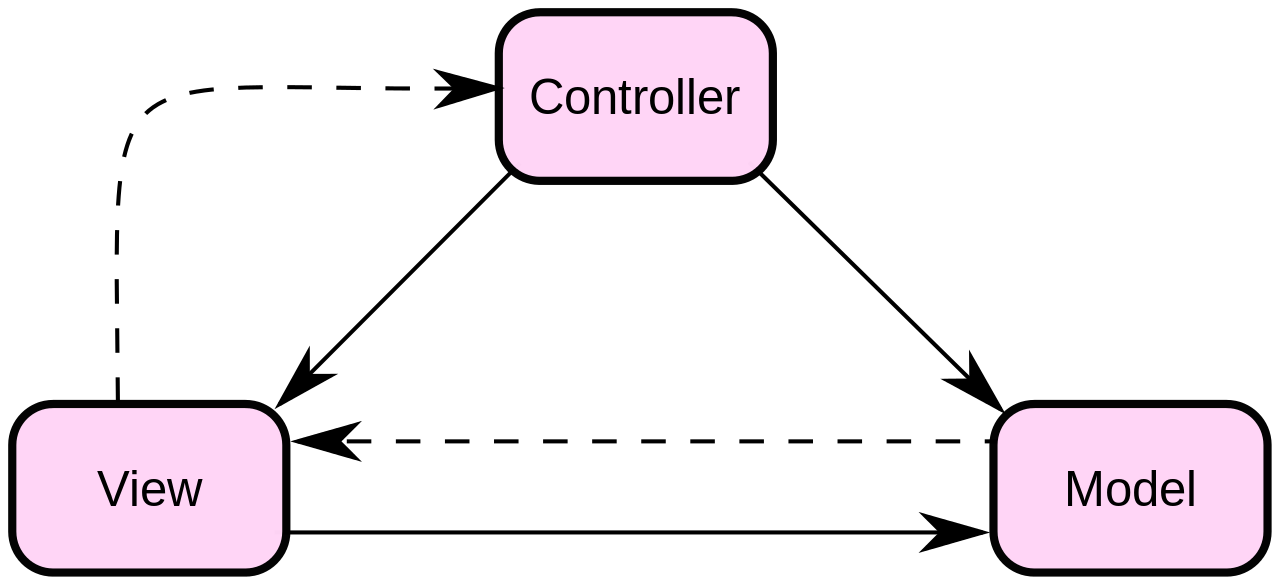
\includegraphics[width=0.9\textwidth]{images/mvc}
		\label{fig:mvc}
		\caption{MVC}
	\end{minipage}
\end{figure}

\begin{figure}[htb]
	\centering
	\begin{minipage}[t]{0.45\linewidth}
		\centering
		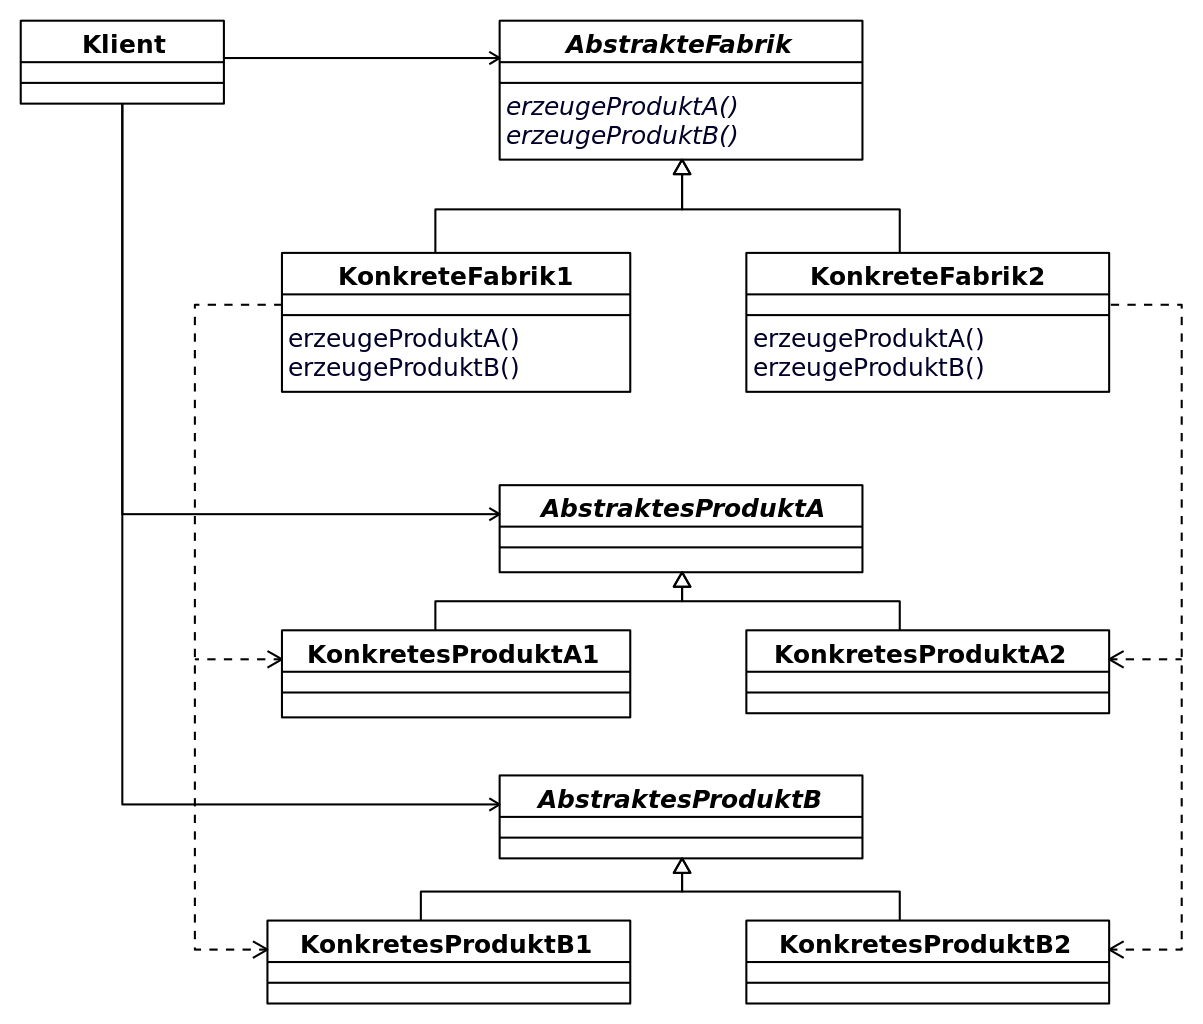
\includegraphics[width=0.9\textwidth]{images/abstract_factory}
		\label{fig:abstract_factory}
		\caption{Abstract Factory}
	\end{minipage}% <- sonst wird hier ein Leerzeichen eingefügt
	\hfill
	\begin{minipage}[t]{0.45\linewidth}
		\centering
		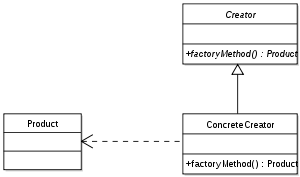
\includegraphics[width=0.9\textwidth]{images/factory}
		\label{fig:factory}
		\caption{Factory}
	\end{minipage}
\end{figure}


\begin{figure}[htb]
	\centering
	\begin{minipage}[t]{0.45\linewidth}
		\centering
		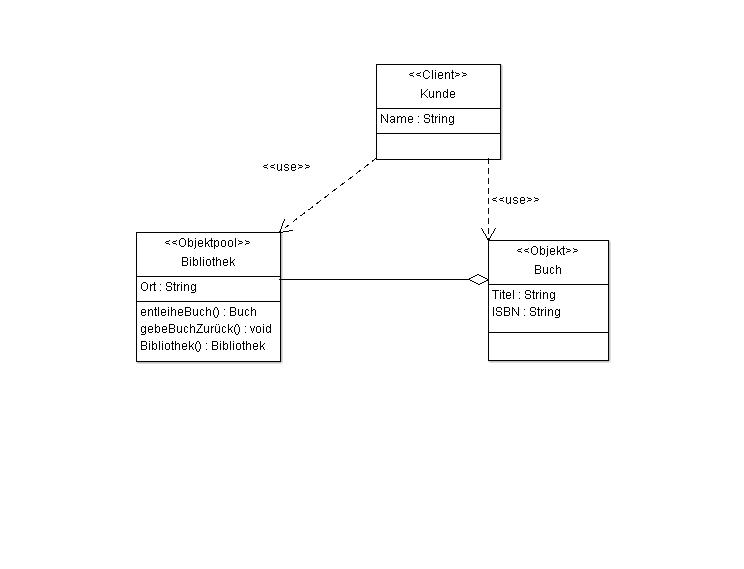
\includegraphics[width=0.9\textwidth]{images/object_pool}
		\label{fig:object_pool}
		\caption{Object Pool}
	\end{minipage}% <- sonst wird hier ein Leerzeichen eingefügt
	\hfill
	\begin{minipage}[t]{0.45\linewidth}
		\centering
		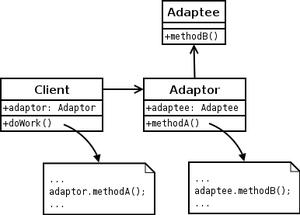
\includegraphics[width=0.9\textwidth]{images/adapter}
		\label{fig:adapter}
		\caption{Adapter}
	\end{minipage}
\end{figure}


\begin{figure}[htb]
	\centering
	\begin{minipage}[t]{0.45\linewidth}
		\centering
		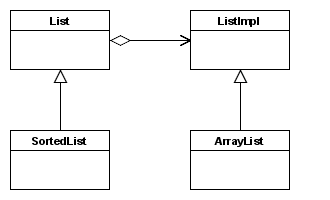
\includegraphics[width=0.9\textwidth]{images/bridge}
		\label{fig:bridge}
		\caption{Bridge}
	\end{minipage}% <- sonst wird hier ein Leerzeichen eingefügt
	\hfill
	\begin{minipage}[t]{0.45\linewidth}
		\centering
		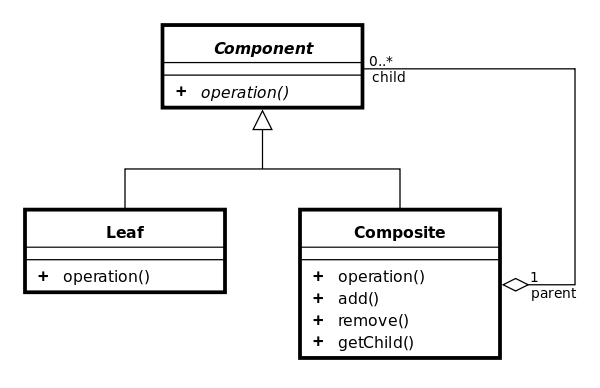
\includegraphics[width=0.9\textwidth]{images/composite}
		\label{fig:composite}
		\caption{Composition}
	\end{minipage}
\end{figure}


\begin{figure}[htb]
	\centering
	\begin{minipage}[t]{0.45\linewidth}
		\centering
		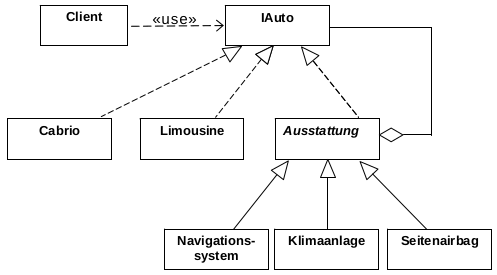
\includegraphics[width=0.9\textwidth]{images/decorator}
		\label{fig:decorator}
		\caption{Decorator}
	\end{minipage}% <- sonst wird hier ein Leerzeichen eingefügt
	\hfill
	\begin{minipage}[t]{0.45\linewidth}
		\centering
		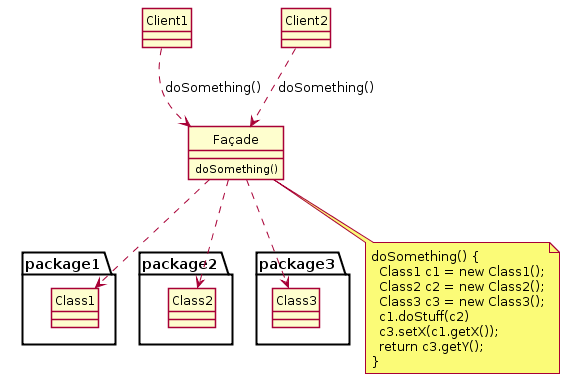
\includegraphics[width=0.9\textwidth]{images/facade}
		\label{fig:facade}
		\caption{Facade}
	\end{minipage}
\end{figure}

\begin{figure}[htb]
	\centering
	\begin{minipage}[t]{0.45\linewidth}
		\centering
		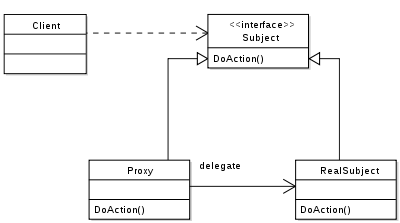
\includegraphics[width=0.9\textwidth]{images/proxy}
		\label{fig:proxy}
		\caption{Proxy}
	\end{minipage}% <- sonst wird hier ein Leerzeichen eingefügt
	\hfill
	\begin{minipage}[t]{0.45\linewidth}
		\centering
		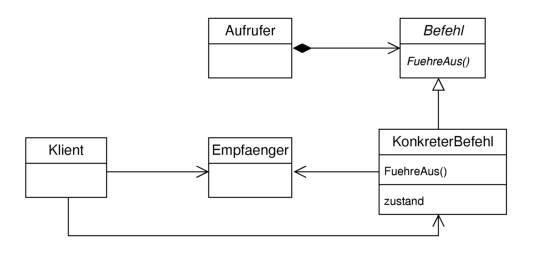
\includegraphics[width=0.9\textwidth]{images/command}
		\label{fig:command}
		\caption{Command}
	\end{minipage}
\end{figure}

\begin{figure}[htb]
	\centering
	\begin{minipage}[t]{0.45\linewidth}
		\centering
		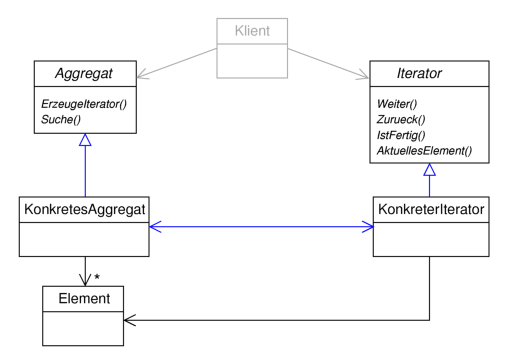
\includegraphics[width=0.9\textwidth]{images/iterator}
		\label{fig:iterator}
		\caption{Iterator}
	\end{minipage}% <- sonst wird hier ein Leerzeichen eingefügt
	\hfill
	\begin{minipage}[t]{0.45\linewidth}
		\centering
		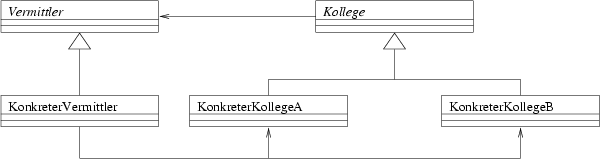
\includegraphics[width=0.9\textwidth]{images/mediator}
		\label{fig:mediator}
		\caption{Mediator}
	\end{minipage}
\end{figure}

\begin{figure}[htb]
	\centering
	\begin{minipage}[t]{0.45\linewidth}
		\centering
		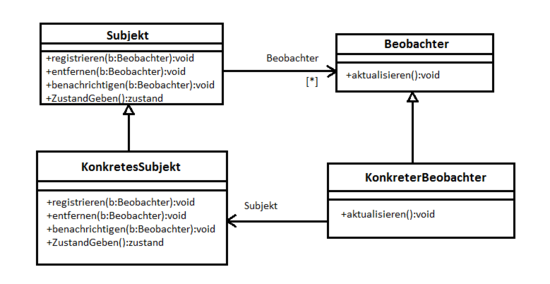
\includegraphics[width=0.9\textwidth]{images/observer}
		\label{fig:observer}
		\caption{Observer}
	\end{minipage}% <- sonst wird hier ein Leerzeichen eingefügt
	\hfill
	\begin{minipage}[t]{0.45\linewidth}
		\centering
		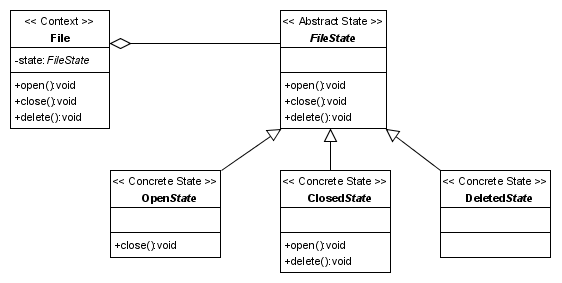
\includegraphics[width=0.9\textwidth]{images/state}
		\label{fig:state}
		\caption{State}
	\end{minipage}
\end{figure}

\begin{figure}[htb]
	\centering
	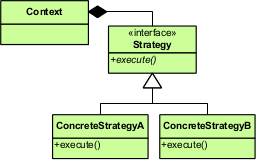
\includegraphics[width=0.7\textwidth]{images/strategy}
	\label{fig:strategy}
	\caption{Strategy}
\end{figure}
\begin{figure}
	\centering
	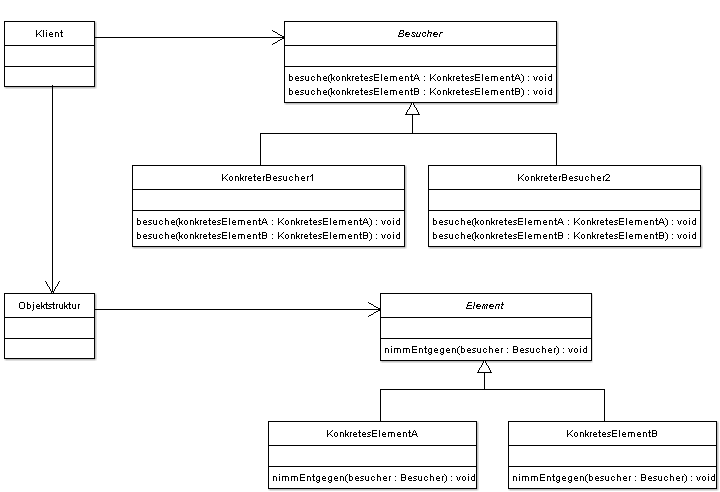
\includegraphics[width=0.7\textwidth]{images/visitor}
	\label{fig:visitor}
	\caption{Visitor}
\end{figure}


